\chapter{DESAIN DAN IMPLEMENTASI}
\label{chap:desainimplementasi}

% Ubah bagian-bagian berikut dengan isi dari desain dan implementasi

Penelitian ini dilaksanakan sesuai dengan sistem berikut dengan implementasinya. Desain sistem merupakan konsep dari pembuatan dan perancangan infrastruktur dan kemudian diwujud kan dalam bentuk blok-blok alur yang harus dikerjakan. Pada bagian implementasi merupakan pelaksanaan teknis untuk setiap blok pada desain sistem.

\section{Deskripsi Sistem}
\label{sec:deskripsisistem}

Sistem pada tugas akhir ini merupakan implementasi dari salah satu disiplin ilmu \textit{Deep Learning} dan pengolahan citra yang berfungsi untuk mendeteksi adanya pejalan kaki yang berada di pinggir jalan, trotoar dan jalur penyebrangan. Selain pejalan kaki, deteksi juga dilakukan pada jalur penyebrangan atau \textit{zebracross} dengan tujuan untuk memberi informasi bahwa disekitar area tersebut terdapat banyak aktivitas pejalan kaki yang menyebrang jalan. Blok diagram metodologi sistem yang digunakan pada penelitian ini dapat dilihat pada Gambar \ref{fig:blok-diagram}.

\begin{figure}[ht]
	\centering
	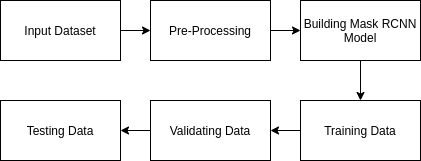
\includegraphics[scale=0.5]{gambar/blok-diagram.png}
	\caption{Blok Diagram Metodologi}
	\label{fig:blok-diagram}
\end{figure}  

\section{Pengumpulan \textit{Dataset} Gambar}
\label{sec:pengumpulandatagambar} 

Pada tugas akhir ini, \textit{dataset} yang digunakan didapatkan dengan beberapa cara, antara lain:
	\begin{enumerate}
		\item \textit{Caltech Pedestrian Database}, merupakan kumpulan gambar yang diambil dari sudut pandang pengendara mobil di California Amerika Serikat dengan ukuran 640 x 480 pixel. Terdapat sekitar 250.000 gambar dengan 350.000 \textit{bounding boxes} dan sekitar 2.300 pejalan kaki dengan kriteria unik diberi tanda. Namun, pada \textit{dataset} ini hanya pejalan kaki saja yang diberi label, sehingga perlu dilakukan proses pelabelan ulang sesuai kelas yang diinginkan. Tidak semua gambar pada \textit{dataset} ini diambil untuk digunakan, gambar yang mempunyai objek berupa pejalan kaki dan \textit{zebracross} saja yang akan digunakan. Gambar \ref{fig:caltech} merupakan contoh dari gambar yang terdapat pada \textit{Caltech Pedestrian Database}.
		\begin{figure}[ht]
			\centering
			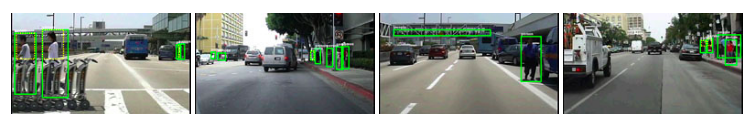
\includegraphics[scale=0.35]{gambar/caltech.png}
			\caption{Contoh Gambar dari Caltech Pedestrian Database}
			\label{fig:caltech}
		\end{figure} 
		
		\item Tangkapan layar dari beberapa video \textit{online Youtube}. Pada cara ini, penulis mencari video yang berada pada salah satu \textit{website video streaming} yaitu Youtube dengan persyaratan video diambil dari sudut pandang pengendara mobil yang berkendara pada jalan raya dengan ukuran gambar 1360x768 px. Pada \textit{frame-frame} tertentu dilakukan \textit{screenshot} dan disimpan untuk selanjutnya dilakukan proses pemberian label pada objek-objek yang diinginkan seperti pada Gambar \ref{fig:youtube-dataset}. 
		
		\begin{figure}[ht]
			\centering
			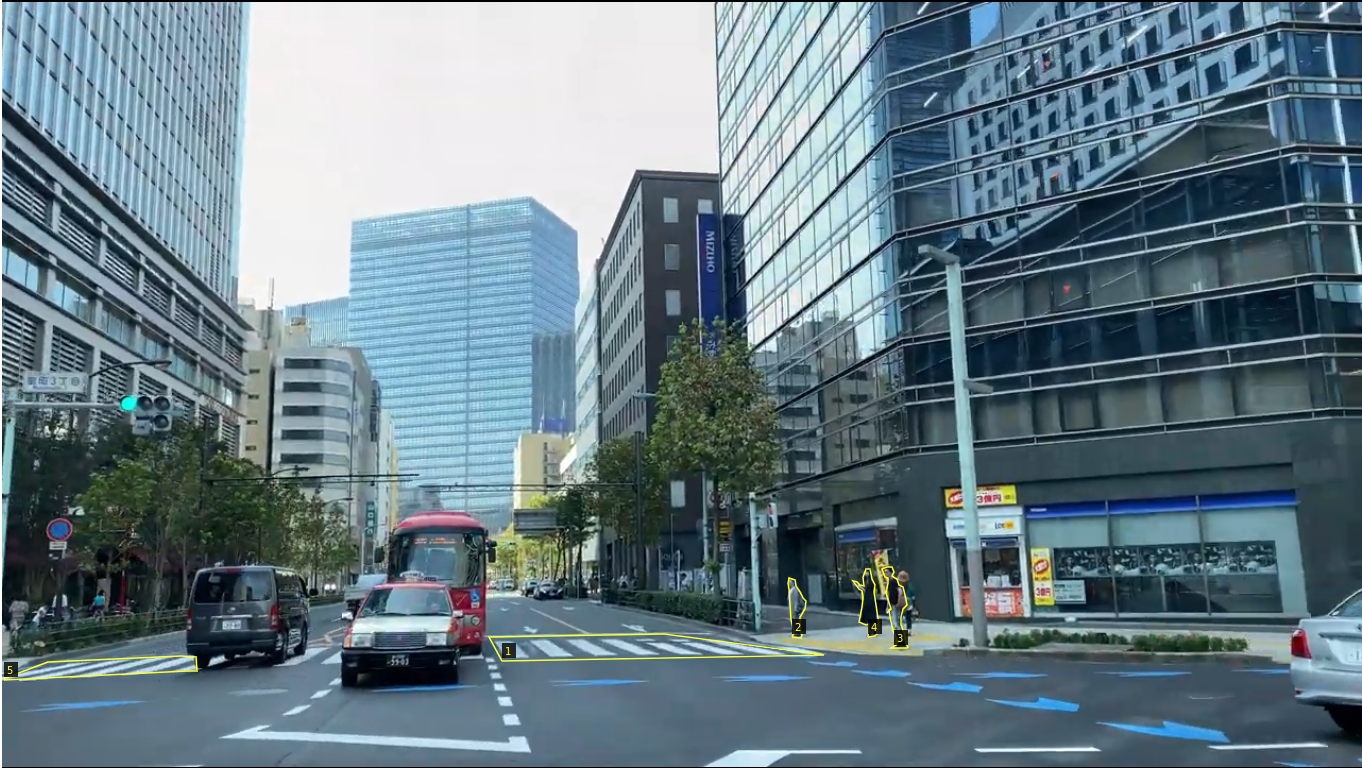
\includegraphics[scale=0.15]{gambar/youtube-dataset.png}
			\caption{Contoh Pembuatan \textit{dataset} dari \textit{Screenshot Youtube}}
			\label{fig:youtube-dataset}
		\end{figure}
		
		\item Pengambilan gambar secara mandiri menggunakan kamera \textit{smartphone} yang diambil dari sudut pandang pengendara motor dengan ukuran gambar yang diambil sebesar 1280x720 px. Pengambilan gambra dilakukan di jalan-jalan Surabaya. Setelah dilakukan pengambilan gambar, proses selanjutnya adalah pemberian label pada objek-objek yang ingin dideteksi.
	\end{enumerate}

\section{Pemisahan Data}
\label{sec:pemisahandata}

Dalam \textit{machine learning} pemisahan data ke beberapa \textit{subset} merupakan suatu hal yang sangat penting. Hal ini dikarenakan setiap \textit{subset} memiliki fungsi masing-masing. Gambar \ref{fig:data-splitting} merupakan rasio pembagian data ke masing-masing subset.

\begin{figure}[ht]
	\centering
	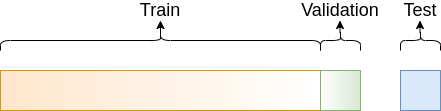
\includegraphics[scale=0.5]{gambar/data-splitting.png}
	\caption{Visualisasi Pembagian Data}
	\label{fig:data-splitting}
\end{figure}

\begin{enumerate}
	\item \textit{Training Sets}\\
	\textit{Training Sets} merupakan sampel data yang digunakan untuk melatih model yang sudah kita buat, dalam bidang \textit{Neural Network} bisa disebut juga bobot dan bias. Model yang sudah kita buat mempelajari pola masukan dan keluaran dari data ini. 
	
	\item \textit{Validation Sets}\\
	\textit{Validation Sets} merupakan sampel data yang digunakan untuk mengevaluasi model yang sudah dilatih menggunakan \textit{training sets}. Selain itu, data ini digunakan untuk memperbarui dan menyempurnakan hyperparameter dari model ke tingkat yang lebih tinggi.
	
	\item\textit{Test Sets}\\
	\textit{Test Sets} merupakan sampel data yang digunakan untuk mengevaluasi model akhir setelah melalui proses \textit{training dan validation}. Apabila pengujian model pada data ini sudah sesuai dengan yang diinginkan, maka proses \textit{learning} sudah selesai. Namun apabila pengujian tidak sesuai dengan yang diharapkan maka diperlukan pengaturan ulang mulai dari proses \textit{training}. 
\end{enumerate}

\section{\textit{Pre-Processing}}
\label{sec:preprocessing}

Pada tahap ini, gambar-gambar dari \textit{dataset} akan mengalami proses penyesuaian sebelum masuk ke proses \textit{data training}.



\section{Implementasi Alat
\label{sec:implementasi alat}}

Alat diimplementasikan dengan \lipsum[1]

% Contoh pembuatan potongan kode
\begin{lstlisting}[
  language=C++,
  caption={Program halo dunia.},
  label={lst:halodunia}
]
#include <iostream>

int main() {
    std::cout << "Halo Dunia!";
    return 0;
}
\end{lstlisting}

\lipsum[2-3]

% Contoh input potongan kode dari file
\lstinputlisting[
  language=Python,
  caption={Program perhitungan bilangan prima.},
  label={lst:bilanganprima}
]{program/bilangan-prima.py}

\lipsum[4]
